% Two-page summary of "What Makes a Latent Fire? Learning Weighted Circuits for Sparse Autoencoder Latents"
% (Linear DAN-216, step 1). DRAFT, 2026-11-15, written from paper/main.tex up to \label{end-of-main}.
% Every number is taken from main.tex; the bracketed pointers (§, Table, Figure) refer to the paper's numbering in
% the build of 2026-11-15 and should be rechecked against the final PDF before the summary is sent.
% Build: latexmk -pdf -outdir=build two-page-summary.tex   (from paper/summary/)
\documentclass[10pt]{article}
\usepackage[a4paper, margin=2cm]{geometry}
\usepackage[T1]{fontenc}
\usepackage{lmodern}
\usepackage{microtype}
\usepackage{graphicx}
\usepackage{amsmath}
\usepackage[hidelinks]{hyperref}
\usepackage{enumitem}
\setlist{nosep, leftmargin=1.3em}
\setlength{\parskip}{0.45em}
\setlength{\parindent}{0pt}
\graphicspath{{../figures/}}
\newcommand{\paperref}[1]{{\small[#1]}}

\begin{document}

\begin{center}
{\Large\bfseries What Makes a Latent Fire?\\[0.15em] Learning Weighted Circuits for Sparse Autoencoder Latents}\\[0.5em]
{\large Daniel Davies (Independent Researcher) \quad Weibo Liu (Brunel University London)}\\[0.3em]
{\small Two-page summary of the paper. Pointers in brackets give the paper section, table or figure for each number.}
\end{center}

\section*{The idea}
Circuit discovery usually explains an output: a logit, a probability, a behavioural metric.
We ask instead what makes an \emph{internal} sparse autoencoder (SAE) latent fire, and build \emph{circuits for latents}.
Targeting latents can capture variables that never show up as a token, and because latents are learned without labels, the model's activations, rather than the tasks we thought to pose, decide what gets explained \paperref{§1}.

\textbf{Weighted circuit masking (WCM).}
For a target latent, every latent at every upstream SAE site is a candidate node.
WCM learns, for each one, a \emph{gate} (is it in the circuit?) and a separate \emph{scaling coefficient} $\alpha$ (how strongly does it act?); the sparsity penalty charges for membership only.
The circuit is trained so that it reproduces the target's pre-activation when every other latent is ablated, under several ablations at once: zero (Z), the latent's sparsity-preserving mean over activating contexts (A) or over contrast contexts (C), and a resample term (R) that takes every non-member latent from a real contrast context, redrawn each step.
The SAE reconstruction errors stay live, and downstream latents are recomputed, not clamped \paperref{§3.1--3.2, Figure~1}.

\textbf{The test.}
A circuit \emph{passes} if, on held-out strongest activating contexts, its faithfulness under Z, A and C each lies in $[0.75, 1.5]$ and its necessity (removing it removes the target) is at least $0.9$.
Sufficiency to induce, a \emph{donor-background test} (everything outside the circuit takes a real donor context's code), and size-matched random circuits given the \emph{same} coefficient fitting are reported but not required \paperref{§3.3}.

\section*{Result 1: circuits for sampled latents, at scale, on three models}
We fit WCM at one sparsity penalty ($\lambda = 10^{-3}$, 400 steps) to $8{,}000$ sampled latents of TuringLLM (12 layers, trained on a documented synthetic corpus) and to $512$ each of Pythia-70m and GPT-2 small with their public Top-K dictionaries; targets are sampled with no prioritisation heuristic \paperref{§4 setup}.
\begin{itemize}
  \item WCM finds a passing circuit for $\mathbf{88.0\%}$ of $7{,}464$ scored TuringLLM targets, $\mathbf{81.9\%}$ of $508$ Pythia-70m and $\mathbf{82.4\%}$ of $511$ GPT-2 small targets, with circuits of a median $609$, $294$ and $371$ upstream latents \paperref{§4.1, Table~1}. Counting unscored and vacuous targets as fails gives $82\%$, $81\%$ and $82\%$.
  \item Size-matched random circuits given the same coefficient fitting pass for none of the $366$ targets tested, while the production circuits of the same targets pass for $83$--$86\%$ \paperref{§4.1}.
  \item Pass rates fall at depth and on weaker contexts: the deepest band passes least ($82.3\%$ at TuringLLM layers 8--11, $65.7\%$ at GPT-2 small layers 8--11), circuits transfer only in part to weaker mid-band contexts ($53.5\%$, $73.6\%$, $66.8\%$), and under real donor backgrounds $69.2\%$, $66.1\%$ and $41.1\%$ still pass \paperref{§4.1}.
  \item The penalty was set on TuringLLM; a size-only rule fixed before a 30-target pilot kept it on both public models. This shows transfer, not optimality \paperref{§4.3}.
\end{itemize}

\section*{Result 2: the coefficients keep circuits small}
Unweighted circuit masking is identical except that every $\alpha$ is fixed at $1$.
On a sweep of $173$ scored TuringLLM targets (eight weighted and five unweighted penalties; Figure~\ref{fig:sweep}):
\begin{itemize}
  \item At layers 8--11, target by target, the smallest passing unweighted circuit is a median $\mathbf{13.8\times}$ larger than the smallest passing weighted one: $\mathbf{6{,}124}$ latents against $\mathbf{436}$, over the $42$ targets both methods pass. This is conservative, since it leaves out targets unweighted masking never passes \paperref{§4.2, Table~14}.
  \item Unweighted circuits peak at $75.1\%$ pass, at a median of $7.6\times10^{4}$ latents, below WCM's $83.2\%$ at $\lambda = 10^{-3}$ \paperref{§4.2, Table~11}.
\end{itemize}
The fitted coefficients are modest (median $1.0$--$1.1$, $80\%$ within $0.7$--$2.2$), yet without them the same nodes almost never pass: setting every coefficient to $1$ drops the pass rate from $88.0\%$ to $1.8\%$ (TuringLLM), $81.9\%$ to $13.8\%$ (Pythia-70m) and $82.4\%$ to $3.3\%$ (GPT-2 small) \paperref{§4.2, Table~13}.
Since random circuits fail under the same fitting, the coefficients make a \emph{selected} node set faithful, not any set.

\begin{figure}[h]
\centering
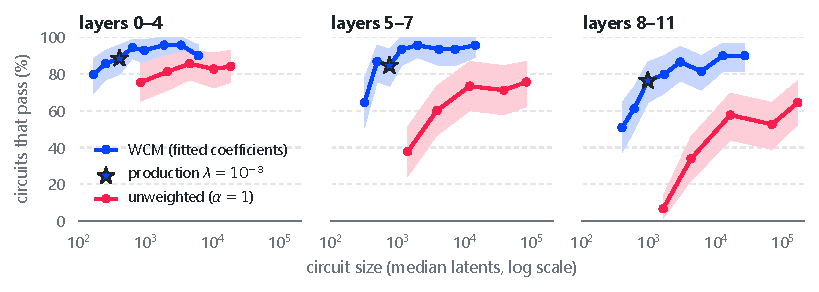
\includegraphics[width=\linewidth]{run2026_tl_sweep_curve.pdf}
\caption{Pass rate against median circuit size on the TuringLLM sweep, by depth band, one point per sparsity penalty: WCM with fitted coefficients (blue) and unweighted circuits, $\alpha = 1$ (red); star, the production penalty $\lambda = 10^{-3}$; shaded, $95\%$ bootstrap bands. Weighted circuits reach each pass rate with fewer latents, and the gap grows with depth \paperref{paper Figure~2}.}
\label{fig:sweep}
\end{figure}

\section*{The main caveat: a circuit is a fitted intervention, not a recovered mechanism}
A WCM circuit acts with the SAE errors kept live, inherits any ambiguity in its latents, and is validated by intervention effects, not against a planted ground truth \paperref{§5.2}.
Its node set is one sample from many near-equivalent solutions: a refit with reordered training contexts passes about as often but shares a median Jaccard of only $0.39$--$0.51$ with the original circuit, so sizes and scores, not memberships, are the properties of a target \paperref{§5}.
A passing circuit can still be read: in the paper's case study, $19$ of the $945$ latents in a circuit for a classical-antiquity latent tell a readable story, and removing them takes the target to $0.22$, $0.10$, $0.21$ under Z, A, C against $0.54$, $0.69$, $0.68$ for as many random members \paperref{§4.4}. But such a reading is an interpretation of an intervention, not proof of the mechanism.

\section*{Why read the paper}
It gives a task-free way to ask what drives \emph{any} latent in an SAE bank, tested under several ablations on held-out text against random circuits that get the same coefficient fitting; it shows that fitted per-node coefficients, not just membership, are what keep such circuits at a few hundred latents; and it states its scope plainly (three models of at most 254M parameters, Top-K dictionaries only, anchors only) \paperref{§5.2}.
A comparison against published attribution baselines on the production run is still pending.
Code: \href{https://github.com/DanielJamesDavies/turing-explorer-circuit-discovery}{\nolinkurl{github.com/DanielJamesDavies/turing-explorer-circuit-discovery}}.

\end{document}
